
\documentclass[border=5pt]{standalone}
\usepackage{xcolor}
\usepackage{tikz}
\usepackage{mathptmx}
\usetikzlibrary{
    positioning,
    calc
}
\tikzset{
    subfig/.style={
        line width = 2.5pt,
        align=center,
        % font=\LARGE
        font=\Huge
    },
}
\def\layerSpace{120mm}

\definecolor{VegetaRed}{HTML}{FFB6C1}
\definecolor{VegetaGreen}{HTML}{7FFFAA}

\begin{document}
    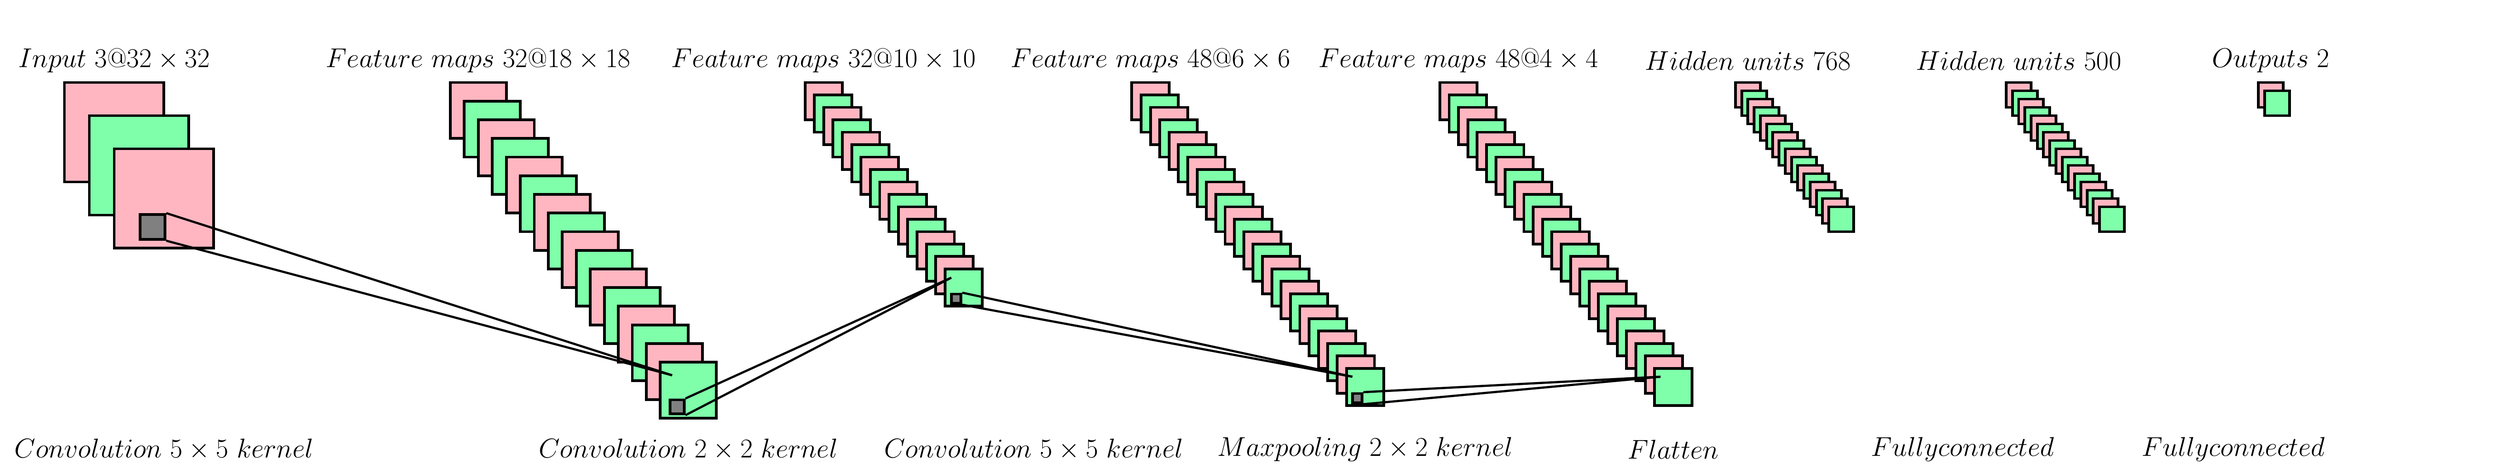
\begin{tikzpicture}
      % \newlength{\mytextlength}

                   \begin{scope}[xshift=0*\layerSpace]
                      % \settowidth{\mytextlength}{$Input~3 @ 32\times 32$}
                       \coordinate (start) at (0,0);
                       \node [subfig,minimum width=32mm, minimum height=32mm] at ($(0,{32mm/2+2em})+(start)$) {$Input~3 @ 32\times 32$};
                       \foreach \i in {1,2,...,3}
                      {
                          \ifodd\i
                              \node [draw,fill=VegetaRed,subfig,minimum width=32mm, minimum height=32mm] at ($({32mm/4*(\i-1)},{-32mm/3*(\i-1)})+ (start)$) {};
                          \else
                              \node [draw,fill=VegetaGreen,subfig,minimum width=32mm, minimum height=32mm] at ($({32mm/4*(\i-1)},{-32mm/3*(\i-1)})+(start)$) {};
                          \fi
                      }
                      % \node (outmap0)[draw,fill=gray,subfig,minimum width=32mm*0.25, minimum height=32mm*0.25] at ($({(32mm/ 4*(3-1)) / 8 * 7},{(-32mm / 3*(3-1)) / 13 * 14})+(start)$) {};
                      \node (outmap0)[draw,fill=gray,subfig,minimum width=32mm*0.25, minimum height=32mm*0.25] at ($({(32mm/ 4*(3-1)) / (1+0.3)},{(-32mm / 3*(3-1)) / (1-0.3)})+(start)$) {};
                    \end{scope}
            
                       \begin{scope}[xshift=1*\layerSpace*(1-1/40)]
                          % \settowidth{\mytextlength}{$Feature~maps~32 @ 18\times 18$}
                           \coordinate (start) at (0,7.0mm);
                           \node [subfig,minimum width=18mm, minimum height=18mm] at ($(0,{18mm/2+2em})+(start)$) {$Feature~maps~32 @ 18\times 18$};
                           \foreach \i in {1,2,...,16.0}
                          {
                              \ifodd\i
                                  \node [draw,fill=VegetaRed,subfig,minimum width=18mm, minimum height=18mm] at ($({18mm/4*(\i-1)},{-18mm/3*(\i-1)})+ (start)$) {};
                              \else
                                  \node [draw,fill=VegetaGreen,subfig,minimum width=18mm, minimum height=18mm] at ($({18mm/4*(\i-1)},{-18mm/3*(\i-1)})+(start)$) {};
                              \fi
                          }
                          \node (outmap1)[draw,fill=gray,subfig,minimum width=18mm*0.25, minimum height=18mm*0.25] at ($({(18mm/ 4*(16.0-1)) / (1+0.05625)},{(-18mm / 3*(16.0-1)) / (1-0.05625)})+(start)$) {};
                          % \node (inmap1)[draw,fill=gray,subfig,minimum width=18mm*0.15, minimum height=18mm*0.15] at ($({(18mm/ 4*(16.0-1)) / (1+0.05625)},{(-18mm / 3*(16.0-1)) / (1+0.05625)})+(start)$) {};
                          \node (inmap1)[subfig] at ($({(18mm/ 4*(16.0-1)) / (1+0.05625)},{(-18mm / 3*(16.0-1)) / (1+0.05625)})+(start)$) {};
                        \end{scope}
                
            \draw [line width=2pt](outmap0.south east) -- (inmap1.west);
            \draw [line width=2pt](outmap0.north east) -- (inmap1.west);
    
                       \begin{scope}[xshift=2*\layerSpace*(1-2/40)]
                          % \settowidth{\mytextlength}{$Feature~maps~32 @ 10\times 10$}
                           \coordinate (start) at (0,10.0mm);
                           \node [subfig,minimum width=12mm, minimum height=12mm] at ($(0,{12mm/2+2em})+(start)$) {$Feature~maps~32 @ 10\times 10$};
                           \foreach \i in {1,2,...,16.0}
                          {
                              \ifodd\i
                                  \node [draw,fill=VegetaRed,subfig,minimum width=12mm, minimum height=12mm] at ($({12mm/4*(\i-1)},{-12mm/3*(\i-1)})+ (start)$) {};
                              \else
                                  \node [draw,fill=VegetaGreen,subfig,minimum width=12mm, minimum height=12mm] at ($({12mm/4*(\i-1)},{-12mm/3*(\i-1)})+(start)$) {};
                              \fi
                          }
                          \node (outmap2)[draw,fill=gray,subfig,minimum width=12mm*0.25, minimum height=12mm*0.25] at ($({(12mm/ 4*(16.0-1)) / (1+0.05625)},{(-12mm / 3*(16.0-1)) / (1-0.05625)})+(start)$) {};
                          % \node (inmap2)[draw,fill=gray,subfig,minimum width=12mm*0.15, minimum height=12mm*0.15] at ($({(12mm/ 4*(16.0-1)) / (1+0.05625)},{(-12mm / 3*(16.0-1)) / (1+0.05625)})+(start)$) {};
                          \node (inmap2)[subfig] at ($({(12mm/ 4*(16.0-1)) / (1+0.05625)},{(-12mm / 3*(16.0-1)) / (1+0.05625)})+(start)$) {};
                        \end{scope}
                
            \draw [line width=2pt](outmap1.south east) -- (inmap2.west);
            \draw [line width=2pt](outmap1.north east) -- (inmap2.west);
    
                       \begin{scope}[xshift=3*\layerSpace*(1-3/40)]
                          % \settowidth{\mytextlength}{$Feature~maps~48 @ 6\times 6$}
                           \coordinate (start) at (0,10.0mm);
                           \node [subfig,minimum width=12mm, minimum height=12mm] at ($(0,{12mm/2+2em})+(start)$) {$Feature~maps~48 @ 6\times 6$};
                           \foreach \i in {1,2,...,24.0}
                          {
                              \ifodd\i
                                  \node [draw,fill=VegetaRed,subfig,minimum width=12mm, minimum height=12mm] at ($({12mm/4*(\i-1)},{-12mm/3*(\i-1)})+ (start)$) {};
                              \else
                                  \node [draw,fill=VegetaGreen,subfig,minimum width=12mm, minimum height=12mm] at ($({12mm/4*(\i-1)},{-12mm/3*(\i-1)})+(start)$) {};
                              \fi
                          }
                          \node (outmap3)[draw,fill=gray,subfig,minimum width=12mm*0.25, minimum height=12mm*0.25] at ($({(12mm/ 4*(24.0-1)) / (1+0.0375)},{(-12mm / 3*(24.0-1)) / (1-0.0375)})+(start)$) {};
                          % \node (inmap3)[draw,fill=gray,subfig,minimum width=12mm*0.15, minimum height=12mm*0.15] at ($({(12mm/ 4*(24.0-1)) / (1+0.0375)},{(-12mm / 3*(24.0-1)) / (1+0.0375)})+(start)$) {};
                          \node (inmap3)[subfig] at ($({(12mm/ 4*(24.0-1)) / (1+0.0375)},{(-12mm / 3*(24.0-1)) / (1+0.0375)})+(start)$) {};
                        \end{scope}
                
            \draw [line width=2pt](outmap2.south east) -- (inmap3.west);
            \draw [line width=2pt](outmap2.north east) -- (inmap3.west);
    
                       \begin{scope}[xshift=4*\layerSpace*(1-4/40)]
                          % \settowidth{\mytextlength}{$Feature~maps~48 @ 4\times 4$}
                           \coordinate (start) at (0,10.0mm);
                           \node [subfig,minimum width=12mm, minimum height=12mm] at ($(0,{12mm/2+2em})+(start)$) {$Feature~maps~48 @ 4\times 4$};
                           \foreach \i in {1,2,...,24.0}
                          {
                              \ifodd\i
                                  \node [draw,fill=VegetaRed,subfig,minimum width=12mm, minimum height=12mm] at ($({12mm/4*(\i-1)},{-12mm/3*(\i-1)})+ (start)$) {};
                              \else
                                  \node [draw,fill=VegetaGreen,subfig,minimum width=12mm, minimum height=12mm] at ($({12mm/4*(\i-1)},{-12mm/3*(\i-1)})+(start)$) {};
                              \fi
                          }
                          % \node (outmap4)[draw,fill=gray,subfig,minimum width=12mm*0.25, minimum height=12mm*0.25] at ($({(12mm/ 4*(24.0-1)) / (1+0.0375)},{(-12mm / 3*(24.0-1)) / (1-0.0375)})+(start)$) {};
                          % \node (inmap4)[draw,fill=gray,subfig,minimum width=12mm*0.15, minimum height=12mm*0.15] at ($({(12mm/ 4*(24.0-1)) / (1+0.0375)},{(-12mm / 3*(24.0-1)) / (1+0.0375)})+(start)$) {};
                          \node (inmap4)[subfig] at ($({(12mm/ 4*(24.0-1)) / (1+0.0375)},{(-12mm / 3*(24.0-1)) / (1+0.0375)})+(start)$) {};
                        \end{scope}
                
            \draw [line width=2pt](outmap3.south east) -- (inmap4.west);
            \draw [line width=2pt](outmap3.north east) -- (inmap4.west);
    
           \begin{scope}[xshift=5*\layerSpace*(1-5/40)]
               \coordinate (start) at (0,12.0mm);
               \node [subfig,minimum width=8mm, minimum height=8mm] at ($(0,{8mm/2+2em})+(start)$) {$Hidden~units~768$};
               \foreach \i in {1,2,...,16}
              {
                  \ifodd\i
                      \node [draw,fill=VegetaRed,subfig,minimum width=8mm, minimum height=8mm] at ($({8mm/4*(\i-1)},{-8mm/3*(\i-1)})+ (start)$) {};
                  \else
                      \node [draw,fill=VegetaGreen,subfig,minimum width=8mm, minimum height=8mm] at ($({8mm/4*(\i-1)},{-8mm/3*(\i-1)})+(start)$) {};
                  \fi
              }
            \end{scope}
    
           \begin{scope}[xshift=6*\layerSpace*(1-6/40)]
               \coordinate (start) at (0,12.0mm);
               \node [subfig,minimum width=8mm, minimum height=8mm] at ($(0,{8mm/2+2em})+(start)$) {$Hidden~units~500$};
               \foreach \i in {1,2,...,16}
              {
                  \ifodd\i
                      \node [draw,fill=VegetaRed,subfig,minimum width=8mm, minimum height=8mm] at ($({8mm/4*(\i-1)},{-8mm/3*(\i-1)})+ (start)$) {};
                  \else
                      \node [draw,fill=VegetaGreen,subfig,minimum width=8mm, minimum height=8mm] at ($({8mm/4*(\i-1)},{-8mm/3*(\i-1)})+(start)$) {};
                  \fi
              }
            \end{scope}
    
           \begin{scope}[xshift=7*\layerSpace*(1-7/40)]
               \coordinate (start) at (0,12.0mm);
               \node [subfig,minimum width=8mm, minimum height=8mm] at ($(0,{8mm/2+2em})+(start)$) {$Outputs~2$};
               \foreach \i in {1,2,...,-6}
              {
                  \ifodd\i
                      \node [draw,fill=VegetaRed,subfig,minimum width=8mm, minimum height=8mm] at ($({8mm/4*(\i-1)},{-8mm/3*(\i-1)})+ (start)$) {};
                  \else
                      \node [draw,fill=VegetaGreen,subfig,minimum width=8mm, minimum height=8mm] at ($({8mm/4*(\i-1)},{-8mm/3*(\i-1)})+(start)$) {};
                  \fi
              }
            \end{scope}
    
           \node [subfig] at ($({16.0mm+0*\layerSpace*(1-0/40)},{-102.0mm})$) {$Convolution~5\times 5~kernel$};

           \node [subfig] at ($({67.5mm+1*\layerSpace*(1-1/40)},{-102.0mm})$) {$Convolution~2\times 2~kernel$};

           \node [subfig] at ($({67.5mm+2*\layerSpace*(1-2/40)},{-102.0mm})$) {$Convolution~5\times 5~kernel$};

           \node [subfig] at ($({69.0mm+3*\layerSpace*(1-3/40)},{-102.0mm})$) {$Maxpooling~2\times 2~kernel$};

           \node [subfig] at ($({69.0mm+4*\layerSpace*(1-4/40)},{-102.0mm})$) {$Flatten$};

           \node [subfig] at ($({69.0mm+5*\layerSpace*(1-5/40)},{-102.0mm})$) {$Fully connected$};

           \node [subfig] at ($({69.0mm+6*\layerSpace*(1-6/40)},{-102.0mm})$) {$Fully connected$};

           \node [subfig] at ($({69.0mm+7*\layerSpace*(1-7/40)},{-102.0mm})$) {$ $};

    \end{tikzpicture}
\end{document}
